\textbf{\underline{OZ 7 - Inductantie - Oefening 4:}}
\vspace{0.5cm}

Op $t = 0$ wordt de open schakelaar gesloten. Toon aan door de regels van Kirchhoff te gebruiken dat de stroom in de spoel op $t > 0$ gelijk is aan:

\begin{equation*}
    I(t) = \frac{\mathcal{E}}{R_1} \left( 1 - e^{-\tfrac{R'}{L}t} \right)
\end{equation*}

waarbij $R' = \frac{R_1R_2}{R_1 + R_2}$.

\begin{center}
    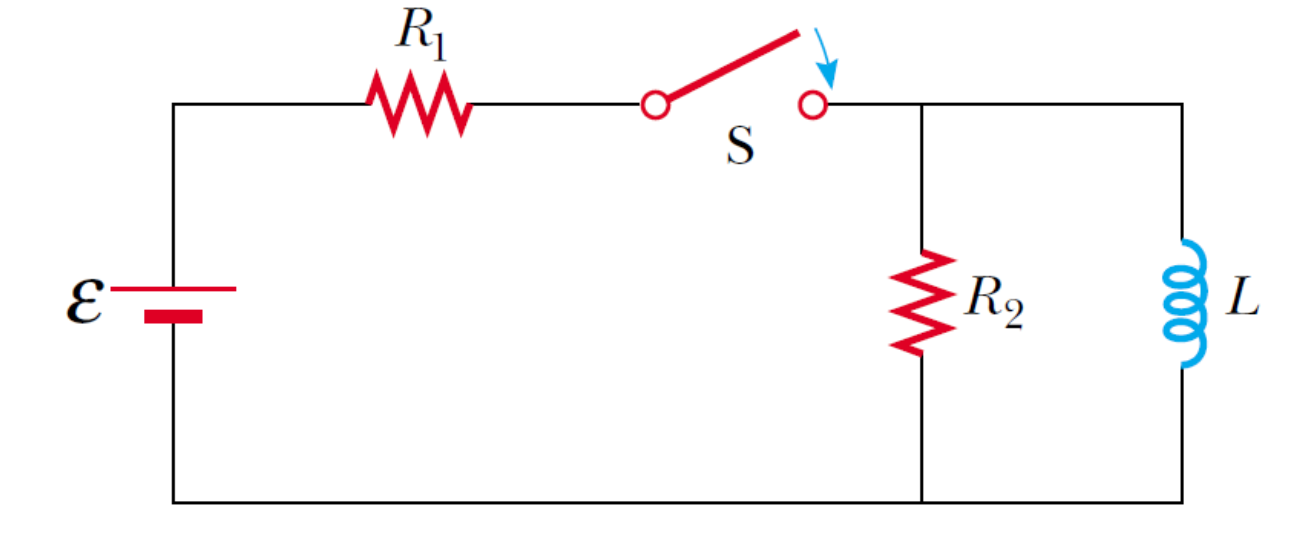
\includegraphics[scale = 0.3]{oz07/resources/Oz7Oef4.png}
\end{center}

\begin{description}[labelwidth=1.5cm, leftmargin=!]
    \item[TB. :] $I(t) = \frac{\mathcal{E}}{R_1} \left( 1 - e^{-\tfrac{R'}{L}t} \right)$ met $R' = \frac{R_1R_2}{R_1 + R_2}$.
    \item[B. :]
        Laat de stromen door $R_1$, $R_2$ en $L$ respectievelijk $I_1$, $I_2$ en $I(t)$ zijn. De knooppuntregel van Kirchhoff geeft
        \begin{equation*}
            I_1 = I_2 + I(t)
        \end{equation*}
        en de spanningsregel in de lussen
        \begin{align}
            \mathcal{E} - (I + I_2)R_1 - I_2R_2 &= 0 \\
            \mathcal{E} - (I + I_2)R_1 -L\frac{dI}{dt} &= 0
        \end{align}
        uit (1) en (2) te combineren volgt
        \begin{equation*}
            I_2 = \frac{L}{R_2} \frac{dI}{dt}.
        \end{equation*}
        We substitueren dit in (1) en krijgen
        \begin{equation*}
            \mathcal{E} - \left(I + \frac{L}{R_2} \frac{dI}{dt} \right)R_1 - \left(\frac{L}{R_2} \frac{dI}{dt}\right)R_2 = 0 
        \end{equation*}
        wat we kunnen herschrijven als
        \begin{equation*}
            \mathcal{E} - IR_1 - \left(\frac{R_1 + R_2 }{R_2} \right)\frac{LdI}{dt} = 0.
        \end{equation*}
        Stel nu $R' = \frac{R_1R_2}{R_1 + R_2}$, dan wordt dit
        \begin{equation*}
            \mathcal{E}' - IR' - \frac{LdI}{dt} = 0.
        \end{equation*}
        waarbij $\mathcal{E}' = \frac{R_2}{R_1+R_2}\mathcal{E} = \frac{R'}{R_1}\mathcal{E}$. De differentiaalvergelijking geeft de oplossing
        \begin{equation*}
            I(t) = \frac{\mathcal{E}'}{R'} \left( 1 - e^{-\tfrac{R'}{L}t} \right)
        \end{equation*}
        wat we kunnen herschrijven als
        \begin{equation*}
            I(t) = \frac{\mathcal{E}}{R_1} \left( 1 - e^{-\tfrac{R'}{L}t} \right)
        \end{equation*}
        waarmee het gevraagde bewezen is.
\end{description}


\vspace{1cm}